\section{固定床反应器的数学模型}


\begin{frame}
    \frametitle{固定床反应器的数学模型}

        \begin{minipage}{0.68\linewidth}
            与均相管式反应器相比，固定床反应器要考虑：
            \begin{itemize}
                \item 器内充填有固体催化剂颗粒，多了一个固相
                \item 相间传递以及在多孔催化剂颗粒内的传递问题
                \item 床层内的轴向传递和径向传递
            \end{itemize}
            
        建立固定床反应器的数学模型时，如将所有这些传递现象都考虑在内，得到的是一组非线性偏微分方程，求解非常困难。需要作合理的简化。
        \end{minipage}\hfill
        \begin{minipage}{0.28\linewidth}
            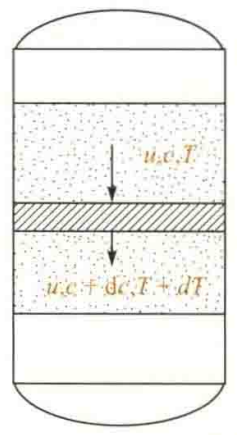
\includegraphics[width=.9\linewidth]{figures/guding.png}
        \end{minipage}

\end{frame}


\begin{frame}
    \frametitle{固定床反应器的数学模型}

    \begin{minipage}{0.68\linewidth}
        绝大多数固定床反应器呈圆柱形，空间变量为两个：
        \begin{itemize}
            \item 轴向变量，轴向浓度和温度梯度必然存在
            \item 径向变量，径向温度和浓度分布也十分明显
        \end{itemize}
        
        若用径向的平均温度和平均浓度分别代替径向温度分布和径向浓度分布，则可将这个典型的二维问题简化为一维问题，于是可用常微分方程来描述。
    \end{minipage}\hfill
    \begin{minipage}{0.28\linewidth}
        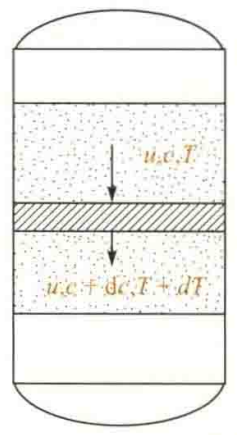
\includegraphics[width=.9\linewidth]{figures/guding.png}
    \end{minipage}

\end{frame}


\begin{frame}
    \frametitle{固定床反应器的数学模型}

    \begin{minipage}{0.68\linewidth}
        流体在固定床内的流动状况与活塞流十分接近，因之可采用活塞流模型。

        取床层高度为d$Z$的微元作组分A的物料衡算可得
        \[
            \frac{G w_{\mathrm{A} 0}}{M_{\mathrm{A}}} \times \frac{\mathrm{d} X_{\mathrm{A}}}{\mathrm{d} Z}=\eta_{0} \rho_{\mathrm{b}}(-\mathscr{R}_{\mathrm{A}})
        \]
        式中$\mathscr{R}_{\mathrm{A}}$为以单位质量催化剂计算的组分A的转化速率。

        大多数工业多相催化反应，相间传递并不显著，因而可以用$\eta$代替$\eta_{0}$，即只考虑内扩散的影响。
    \end{minipage}\hfill
    \begin{minipage}{0.28\linewidth}
        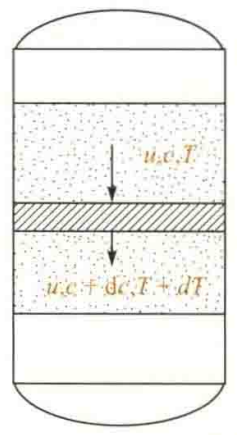
\includegraphics[width=.9\linewidth]{figures/guding.png}
    \end{minipage}

\end{frame}


\begin{frame}
    \frametitle{固定床反应器的数学模型}

    如果不考虑轴向热扩散，对此微元体积作热量衡算则有
    \[
        G C_{p \mathrm{t}} \frac{\mathrm{d} T}{\mathrm{d} Z}=\eta_{0} \rho_{\mathrm{b}}(-\mathscr{R}_{\mathrm{A}})(-\Delta H_{\mathrm{r}})-\frac{4 U}{d_{\mathrm{t}}}(T-T_{\mathrm{c}})
    \]
    流体流过床层时压力变化太大的话，还需建立一动量衡算式，即压力分布方程
    \[
        -\frac{\mathrm{d} p}{\mathrm{~d} Z}=\frac{f G^{2}(1-\varepsilon)}{\rho d_{\mathrm{p}} \varepsilon^{3}}
    \]
    初值条件为$Z=0, \quad X_{\mathrm{A}}=0, \quad T=T_{0}, \quad P=P_{0}$

    冷却介质温度$T_{\mathrm{C}}$如果不能视作常数，则还需冷却介质温度的轴向分布方程
    \[
        G_{\mathrm{C}} C_{p \mathrm{c}} \frac{\mathrm{d} T_{\mathrm{C}}}{\mathrm{d} Z}=\frac{4 U}{d_{\mathrm{t}}}(T-T_{\mathrm{C}})
    \]
    初值条件为$Z=0, \quad T_{\mathrm{C}}=T_{\mathrm{C} 0}$

\end{frame}


\begin{frame}
    \frametitle{固定床反应器的数学模型}

    通过求解这些式子，便可回答固定床反应器设计中的一个最重要的问题，即达到规定的转化率需要多高的催化剂床层。可根据不同情况简化。

    \begin{itemize}
        \item 等温情况
            \begin{itemize}
                \item 物料衡算式
            \end{itemize}        
        \item 非等温情况
            \begin{itemize}
                \item 物料衡算式
                \item 能量衡算式
            \end{itemize} 
        \item 高压下反应且压力降又较大时
        \begin{itemize}
            \item 物料衡算式
            \item 能量衡算式
            \item 动量衡算式
        \end{itemize}
    \end{itemize}

\end{frame}


\begin{frame}
    \frametitle{固定床反应器的数学模型}

    若为多个反应，上述方程中涉及到反应速率项的需作适当的改写。
    
    物料衡算式：
    \[
        \frac{\mathrm{d}(u_{0} c_{i})}{\mathrm{d} Z}=\rho_{\mathrm{b}} \sum_{j=1}^{M} \eta_{j} \nu_{i j} \bar{r}_{j} \qquad(i=1,2, \cdots, k)
    \]
    热量衡算式：
    \[
        u_{0} C_{p \mathrm{t}} \rho_{\mathrm{f}} \frac{\mathrm{d} T}{\mathrm{d} Z}=\rho_{\mathrm{b}} \sum_{j=1}^{k} \eta_{j}\left|\nu_{i j}\right| \bar{r}_{j}(-\Delta H_{\mathrm{r}})_{j}-\frac{4 U}{d_{\mathrm{t}}}(T-T_{\mathrm{c}})
    \]
    相应的初值条件为：$Z=0,  \quad T=T_{0}, \quad c_{i}=c_{i0} \quad (i=1,2, \cdots, k)$

\end{frame}


\begin{frame}
    \frametitle{固定床反应器的数学模型}

    固定床床层太薄时，活塞流的假定不成立。此时需考虑返混的影响，恒容情况下进行单一反应时固定床反应器的模型方程为
    \[
        \varepsilon D_{\mathrm{a}} \frac{\mathrm{d}^{2} c_{\mathrm{A}}}{\mathrm{d} Z^{2}}-u_{0} \frac{\mathrm{d} c_{\mathrm{A}}}{\mathrm{d} Z}-\eta_{0} \rho_{\mathrm{b}}(-\mathscr{R}_{\mathrm{A}})=0 
    \]
    热量衡算式：
    \[
        \lambda_{\mathrm{ea}} \frac{\mathrm{d}^{2} T}{\mathrm{d} Z^{2}}-\rho_{\mathrm{f}} u_{0} C_{p \mathrm{t}} \frac{\mathrm{d} T}{\mathrm{d} Z}+\eta_{0} \rho_{\mathrm{b}}(-\mathscr{R}_{\mathrm{A}})(-\Delta H_{\mathrm{r}})-\frac{4 U}{d_{\mathrm{t}}}(T-T_{\mathrm{C}})=0
    \]
    边界条件：
    \[
        Z=0, u_{0}(C_{\mathrm{A} 0}-C_{\mathrm{A}})=-\varepsilon D_{\mathrm{a}} \frac{\mathrm{d} c_{\mathrm{A}}}{\mathrm{d} Z}
    \]
    \[
        u_{0} \rho_{\mathrm{f}} C_{p \mathrm{t}}(T_{0}-T)=\lambda_{\varepsilon \mathrm{a}} \frac{\mathrm{d} T}{\mathrm{~d} Z} \qquad Z=L, \quad \frac{\mathrm{d} c_{\mathrm{A}}}{\mathrm{d} Z}=\frac{\mathrm{d} T}{\mathrm{~d} Z}=0
    \]

\end{frame}


\begin{frame}
    \frametitle{固定床反应器的数学模型}

    模型方程变为二阶常微分方程，即在活塞流模型方程的基础上叠加一轴向扩散项。
    
    显然，对属于正常动力学的反应，返混的存在将会使转化率降低。

    上述模型方程的应用，需要具备三类基础数据。
    \begin{itemize}
        \item 动力学数据；
        \item 热力学数据；
            \begin{itemize}
                \item 如反应热、比热容、化学平衡常数等等。
            \end{itemize}
        \item 传递速率数据
            \begin{itemize}
                \item 包括流体的传递性质，如黏度、扩散系数和导热系数等。
                \item 催化剂的宏观结构数据，如孔分布、颗粒密度、堆密度和比表面等。
            \end{itemize}
    \end{itemize}

\end{frame}